\documentclass[12pt]{article}
\usepackage[utf8]{inputenc}
\usepackage[margin=2.54cm]{geometry}
\usepackage[titletoc,title]{appendix}
\usepackage{amsmath,amsfonts,amssymb,mathtools,amsthm}

\usepackage{graphicx,float}
\graphicspath{{images/}}

\usepackage{tikz}
\usepackage{tikz-3dplot, subcaption}
\usetikzlibrary{angles,quotes,calc}

\usepackage[maxbibnames=99]{biblatex}
\addbibresource{references.bib}

\theoremstyle{plain}
\newtheorem{thm}{Theorem}[section] 
\newtheorem{prop}[thm]{Proposition}
\newtheorem{lem}[thm]{Lemma}
\newtheorem{cor}[thm]{Corollary}

\theoremstyle{definition}
\newtheorem{defn}[thm]{Definition}
\newtheorem{ex}[thm]{Example}

\title{Rotations and Quaternions: \\
    \large A Motivated Introduction\thanks{MATH381W Term Project.}}
\author{Scott Renegado\\ Department of Mathematics, Simon Fraser University, Burnaby, B.C., Canada\\ \tt{srenegad@sfu.ca} }
\date{}

\begin{document}

\maketitle

\begin{abstract}
In this paper, we introduce quaternions with intent to give readers a greater appreciation for them. We first explore the complex numbers as an analog to quaternions, and how they relate to two-dimensional rotations. From there, we meet the quaternions and their relation to three-dimensional rotations. A simple geometric interpretation that visualizes multiplication of unit quaternions on the unit three-sphere is provided \cite{hanson}. In the end, we point to different resources that the reader may see fit to dabble in. An undergraduate linear algebra refreshment is recommended, but not needed.\footnote{See these books \cite{anton, axler}.}
\end{abstract}

\section{Introduction}
In the mid-nineteenth century, Sir William Rowan Hamilton was taking a leisurely stroll with his wife along the Royal Canal in Dublin. As if an electric circuit had finally closed, Hamilton came up with the idea of \textit{quaternions} -- a four-dimensional extension of the real numbers defined with the following fundamental multiplication rule:  
\begin{equation*}
    \textit{i}^2 = \textit{j}^2 = \textit{k}^2 = \textit{ijk} = -1.
\end{equation*}
His discovery led to defacing public property, as he carved into the side of the Broome Bridge the equation with a knife \cite{hanson}. 

History aside, we note that quaternions have surprisingly found applications in computer graphics and animation, particularly in describing three-dimensional rotations \cite{goldman, hanson}. It turns out quaternion multiplication provide an efficient method in computing three-dimensional rotations, in terms of speed, storage, and avoidance of numerical inaccuracies \cite{goldman}.

\section{Complex Numbers}
\label{complex}

\subsection{Basic Definition and Properties}
\label{complexDefn}

Before learning quaternions, we first, assuming familiarity with the real numbers, define the complex numbers.
\begin{defn} \label{compDefn}
A \textbf{\textit{complex number}} is an ordered pair $(a,b)$ where $a,b \in \mathbb{R}$. 
\begin{itemize}
    \item Let $i$ denote the complex number $(0,1)$. Instead of writing a complex number as $(a,b)$, we write $a+bi$.
    \item Let $z$ denote a complex number so that $z = a+bi$. We denote Re $z=a$, the \textbf{\textit{real part of z}} and Im $z=b$, the \textbf{\textit{imaginary part of z}}. If Re $z=a=0$, $z$ is called an \textbf{\textit{imaginary number}}. If Im $z=b=0$, then $z$ is identified with a real number.
    \item The set of complex numbers is denoted by $\mathbb{C}$ where
    \begin{equation*}
        \mathbb{C} = \{a+bi : a,b \in \mathbb{R} \}.
    \end{equation*}
    \item Let $z_1 = a+bi$, $z_2 = c+di\in\mathbb{C}$. \textbf{\textit{Addition}} and \textbf{\textit{multiplication}} on $\mathbb{C}$ is defined by:
    \begin{align*}
        z_1 + z_2 &= (a+bi) + (c+di) = (a+c) + (b+d)i \\
        z_1z_2 &= (a+bi)(c+di) = (ac-bd) + (ad+bc)i
    \end{align*}
    \item Let $z=a+bi\in\mathbb{C}$. The \textbf{\textit{complex conjugate}} of $z$ is denoted by $\overline{z}$ or $z^*$ where $\overline{z}=a-bi$. The \textbf{\textit{modulus}} or \textbf{\textit{absolute value}} of $z$ is denoted by $|z|$ where $|z|=\sqrt{\overline{z}z}=\sqrt{a^2+b^2}$. A complex number with modulus 1 is a \textbf{\textit{unit complex number}}. 
 \end{itemize}
\end{defn}

Note that from the multiplication rule, check that 
\begin{align*}
    i^2 = -1.
\end{align*}
We never really need to memorize the multiplication rule. Instead, knowing $i^2=-1$ and the usual rules for real arithmetic makes complex multiplication rather straightforward.

In the next proposition, we provide basic algebraic properties. Glancing over its proof and the details, which can be found, for example, in the beginning sections of the books \cite{axler, brown} (that also go into further properties), we shift our focus over to vectors in $\mathbb{R}^2$.

\begin{prop}
(Basic Algebraic Properties) 
\begin{itemize}
    \item Addition and multiplication on $\mathbb{C}$ are \textbf{associative} and \textbf{commutative}.
    \item The \textbf{additive identity} is 0+0i = 0 and the \textbf{multiplicative identity} is 1+0i = 1.
    \item Every complex number has a unique \textbf{additive inverse} and unique \textbf{multiplicative inverse}.
    \item Multiplication \textbf{distributes} over addition.
\end{itemize}

\end{prop}

\subsection{Identification with Vectors}
\label{compIden}
As complex numbers are ordered pairs of real numbers, it is natural to identify complex numbers with points or vectors in $\mathbb{R}^2$.

\begin{defn} \label{compDefnVec}
The complex numbers $\mathbb{C}$ is a two-dimensional \textit{vector space} over $\mathbb{R}$. We say $\mathbb{C}$ is isomorphic to $\mathbb{R}^2$, and write $\mathbb{C}\cong \mathbb{R}^2$.
\begin{itemize}
    \item Geometrically, $z=a+bi$ corresponds to a point in the \textbf{\textit{complex plane}} with rectangular coordinates $a$ and $b$. The complex plane is identified with the $xy$-plane, where the axis identified with the $x$-axis is called the \textbf{\textit{real axis}}, while the axis identified with the $y$-axis is the \textbf{\textit{imaginary axis}}. The vector emanating from the origin to the point $(a,b)$ is identified with $z$. We interchangeably refer to $z$ as a point or vector.
    \item The \textbf{\textit{standard basis}} is \{1,i\} where 1 is identified with the unit vector along the positive $x$-axis, and $i$ is identified with the unit vector along the positive $y$-axis.
\end{itemize}
\end{defn}

This gives us a geometric interpretation -- we can use the parallelogram rule for vector addition when adding (or subtracting) two complex numbers; similarly, multiplying a complex number $z$ by a real number $c$ corresponds to scaling the vector $z$ by $c$.

\numberwithin{figure}{section}
\begin{figure}[h]
    \centering
    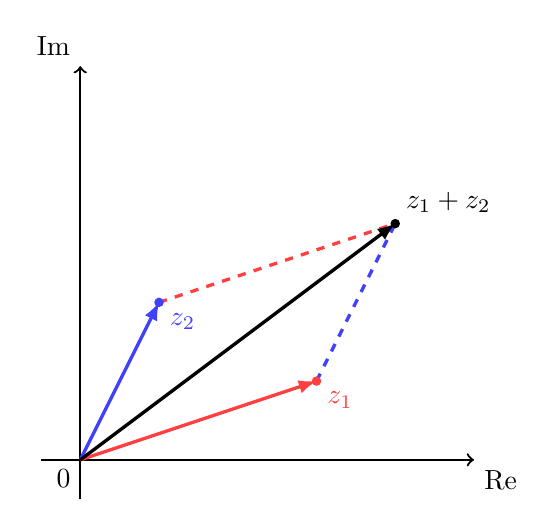
\begin{tikzpicture}
        %\draw[step=1cm,gray,very thin] (-1.9, -1.9) grid (5.9, 5.9);
        
        % Axis.
        \draw[thick, ->] (-0.5,0) -- (5,0) node[below right] {Re};
        \draw[thick, ->] (0,-0.5) -- (0,5) node[above left] {Im};
        \filldraw[black] (0, 0) node[below left] {$0$};
        
        \draw[red!75, very thick, -latex] (0,0) -- (3,1) node[below right] {$z_1$};
        \draw[blue!75, very thick, -latex] (0,0) -- (1,2) node[below right] {$z_2$};
        \draw[red!75, very thick, dashed] (1,2) -- (4,3);
        \draw[blue!75, very thick, dashed] (3,1) -- (4,3);
        \filldraw[red!75] (3, 1) circle (1.5pt);
        \filldraw[blue!75] (1, 2) circle (1.5pt);
        \draw[very thick, -latex] (0,0) -- (4,3) node[above right] {$z_1+z_2$};
        \filldraw[black] (4, 3) circle (1.5pt);
    \end{tikzpicture}
    \begin{tikzpicture}
        %\draw[step=1cm,gray,very thin] (-1.9, -1.9) grid (5.9, 5.9);
        
        % Axis.
        \draw[thick, ->] (-0.5,0) -- (5,0) node[below right] {Re};
        \draw[thick, ->] (0,-0.5) -- (0,5) node[above left] {Im};
        \filldraw[black] (0, 0) node[below left] {$0$};
        
        \draw[red!75, very thick, -latex] (0,0) -- (4,4) node[below right] {$cz$};
        \draw[very thick, -latex] (0,0) -- (2,2) node[below right] {$z$};
        \filldraw[red!75] (4, 4) circle (1.5pt);
        \filldraw[black] (2, 2) circle (1.5pt);

    \end{tikzpicture}
    \caption{Complex addition (and subtraction) interpreted as vector addition (and subtraction). Multiplying a real number with a complex number interpreted as scalar multiplication.}
    \label{fig:arithmetic}
\end{figure}

When we multiply two complex numbers, notice that this defines a \textit{linear map} or \textit{linear transformation} on $\mathbb{C}$ because if $w,z_1,z_2\in \mathbb{C}$ and $c_1,c_2\in \mathbb{R}$, then since multiplicative is commutivative and distributes over addition,
\begin{align*}
w(c_1z_1 + c_2z_2) &= c_1wz_1 + c_2wz_2.
\end{align*}
Suppose $w$ is a unit complex number. Multiplying by $w$ preserves the modulus of $z$ since $|w|=1$ and so $|wz_1|=|z_1|$.\footnote{A property we glanced over is that if $z_1,z_2 \in \mathbb{C}$, then $|z_1z_2|=|z_1||z_2|$ \cite{anton}.} So multiplying by a unit complex number is an \textit{orthogonal linear transformation} on $\mathbb{R}^2 \cong \mathbb{C}$, which are exactly rotations about the origin \cite{axler}!

We understand this better when considering complex numbers in polar coordinates.

\begin{defn}
Let $z=a+bi\in \mathbb{C}$ be nonzero, and let $r,\theta$ be the polar coordinates corresponding to the point $(a,b)$. Then $z$ can be written in \textbf{\textit{polar form}} as
\begin{align*}
    z = r(\cos\theta + i\sin\theta)
\end{align*}
where $r=|z|$. A value of $\theta$ is called an \textbf{\textit{argument}} of $z$. If $-\pi<\theta \leq \pi$, then $\theta$ is a \textbf{\textit{principal value}}.\footnote{We can compactly write the polar form of a complex number $z=r(\cos\theta+i\sin\theta)$ by using \textit{Euler's Formula}, $e^{i\theta}=cos\theta + isin\theta$, so that $z=re^{i\theta}$. More details can be found in \cite{brown}.} 
\end{defn}

\numberwithin{figure}{section}
\begin{figure}[h]
    \centering
    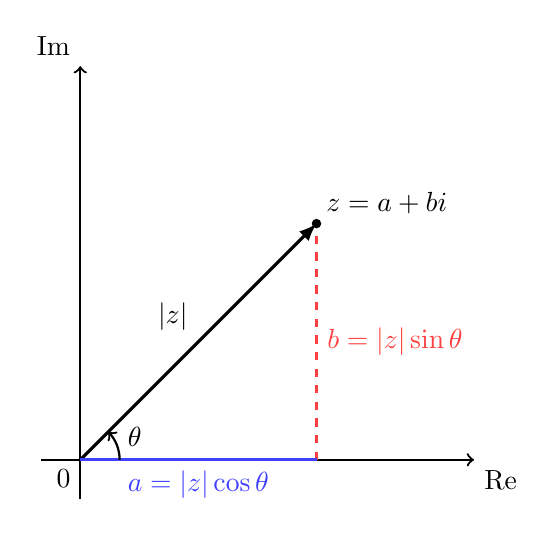
\begin{tikzpicture}
        %\draw[step=1cm,gray,very thin] (-1.9, -1.9) grid (5.9, 5.9);
        \coordinate (O) at (0,0);
        \coordinate (A) at (3,0);
        \coordinate (Z) at (3,3);
        
        % Axis.
        \draw[thick, ->] (-0.5,0) -- (5,0) node[below right] {Re};
        \draw[thick, ->] (0,-0.5) -- (0,5) node[above left] {Im};
        \filldraw[black] (0,0) node[below left] {$0$};
        
        \draw[red!75,very thick, dashed] (3,0) -- node[right] {$b=|z|\sin\theta$} ++ (0,3);
        \draw[very thick, -latex] (0,0) -- node[above left] {$|z|$} ++ (3,3);
        \draw[blue!75,very thick] (0,0) -- node[below] {$a=|z|\cos\theta$} ++ (3,0);
        \filldraw[black] (3, 3) circle (1.5pt) node[above right] {$z=a+bi$};
        
        \pic[draw, thick, ->, "$\theta$", angle eccentricity=1.5] {angle=A--O--Z};
        
    \end{tikzpicture}
    \caption{Geometry of $z=a+bi\in \mathbb{C}$.}
    \label{fig:polarComplex}
\end{figure}

Let $z_1 = |z_1|(\cos\theta_1 + i\sin\theta_1), z_2 = |z_2|(\cos\theta_2+i\sin\theta_2) \in \mathbb{C}$. Multiplying the two and applying trigonometric identities (sum formulas), we get
\begin{align*}
    z_1z_2 &= |z_1||z_2|(\cos\theta_1 + i\sin\theta_1)(\cos\theta_2+i\sin\theta_2) \\
        &= |z_1||z_2|[(\cos\theta_1\cos\theta_2 - \sin\theta_1\sin\theta_2) + i(\cos\theta_1\sin\theta_2 + \cos\theta_1\sin\theta_1)] \\
        &= |z_1||z_2|[\cos(\theta_1 + \theta_2) + i\sin(\theta_1+\theta_2)].
\end{align*}

\numberwithin{figure}{section}
\begin{figure}[h]
    \centering
    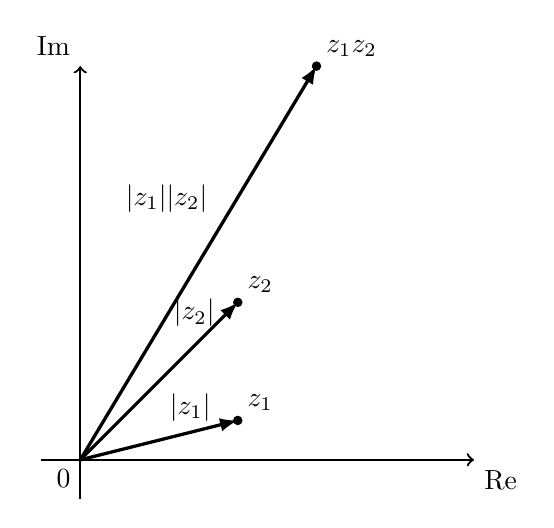
\begin{tikzpicture}
        %\draw[step=1cm,gray,very thin] (-1.9, -1.9) grid (5.9, 5.9);
        \coordinate (O) at (0,0);
        \coordinate (A1) at (2,0);
        \coordinate (Z1) at (2,0.5);
        \coordinate (A2) at (2,0);
        \coordinate (Z2) at (2,2);
        \coordinate (A12) at (3,0);
        \coordinate (Z12) at (3,5);
        
        % Axis.
        \draw[thick, ->] (-0.5,0) -- (5,0) node[below right] {Re};
        \draw[thick, ->] (0,-0.5) -- (0,5) node[above left] {Im};
        \filldraw[black] (0,0) node[below left] {$0$};
        
        %z_1
        \draw[very thick, -latex] (O) -- node[above right, yshift=1mm] {$|z_1|$} ++ (Z1);
        \filldraw[black] (Z1) circle (1.5pt) node[above right] {$z_1$};

        %z_2
        \draw[very thick, -latex] (O) -- node[above right, yshift=5.5mm, xshift=0.5mm] {$|z_2|$} ++ (Z2);
        \filldraw[black] (Z2) circle (1.5pt) node[above right] {$z_2$};

        %z_1z_2
        \draw[very thick, -latex] (O) -- node[above left, yshift=5mm, xshift=2.5mm] {$|z_1||z_2|$} ++ (Z12);
        \filldraw[black] (Z12) circle (1.5pt) node[above right] {$z_1z_2$};

    \end{tikzpicture}    
    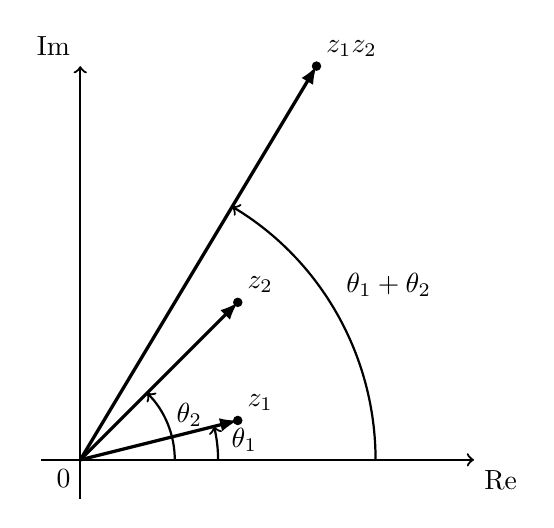
\begin{tikzpicture}
        %\draw[step=1cm,gray,very thin] (-1.9, -1.9) grid (5.9, 5.9);
        \coordinate (O) at (0,0);
        \coordinate (A1) at (2,0);
        \coordinate (Z1) at (2,0.5);
        \coordinate (A2) at (2,0);
        \coordinate (Z2) at (2,2);
        \coordinate (A12) at (3,0);
        \coordinate (Z12) at (3,5);
        
        % Axis.
        \draw[thick, ->] (-0.5,0) -- (5,0) node[below right] {Re};
        \draw[thick, ->] (0,-0.5) -- (0,5) node[above left] {Im};
        \filldraw[black] (0,0) node[below left] {$0$};
        
        %z_1
        \draw[very thick, -latex] (O) -- (Z1);
        \filldraw[black] (Z1) circle (1.5pt) node[above right] {$z_1$};
        \pic[draw, thick, ->, "$\theta_1$", angle radius = 1.75cm, angle eccentricity=1.2] {angle=A1--O--Z1};
        
        %z_2
        \draw[very thick, -latex] (O) --  (Z2);
        \filldraw[black] (Z2) circle (1.5pt) node[above right] {$z_2$};
        \pic[draw, thick, ->, "$\theta_2$", angle radius = 1.2cm,  angle eccentricity=1.25] {angle=A2--O--Z2};
        
        %z_1z_2
        \draw[very thick, -latex] (O) -- (Z12);
        \filldraw[black] (Z12) circle (1.5pt) node[above right] {$z_1z_2$};
        \pic[draw, thick, ->, "$\theta_1+\theta_2$", angle radius = 3.75cm, angle eccentricity=1.2] {angle=A12--O--Z12};

    \end{tikzpicture}
    \caption{The product $z_1z_2$ represents the vector $z_2$ ($z_1$)  scaled by $|z_1|$ ($|z_2|$) and rotated counterclockwise about the origin by $\theta_1$ ($\theta_2$).}
    \label{fig:complexRot}
\end{figure}
From Figure \ref{fig:complexRot}, we see the geometric effect of  complex multiplication in the complex plane! 

We conclude this section by making a connection to the unit circle, $S^1$, i.e.
\begin{align*}
    S^1 = \{(x,y)\in\mathbb{R}^2 : x^2+y^2=1\}.
\end{align*}
It follows that a point in $S^1$ corresponds to a unit complex number, $z=a+bi$, since  $|z|^2=a^2+b^2=1$. Furthermore, because unit complex numbers have modulus 1, by the polar form of complex numbers, multiplying two unit complex numbers produces back a unit complex number.

\begin{figure}[h]
    \centering
    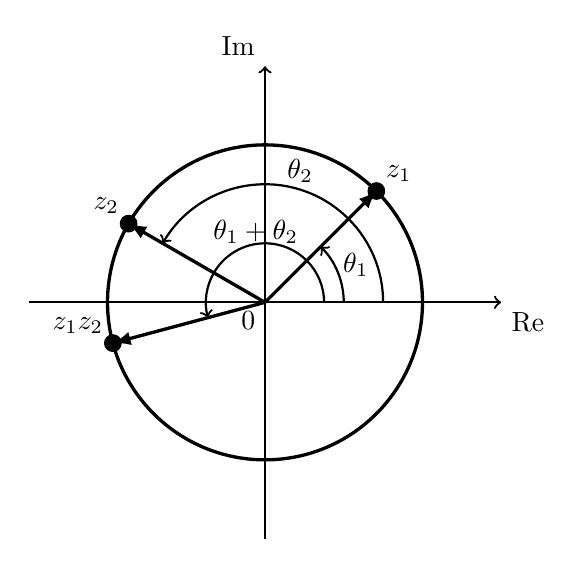
\begin{tikzpicture}[scale=2]
        %\draw[step=1cm,gray,very thin] (-1.9, -1.9) grid (5.9, 5.9);
        \coordinate (O) at (0,0);
        \coordinate (A1) at ($1/sqrt(2)*(1,0)$);
        \coordinate (Z1) at ($1/sqrt(2)*(1,1)$);
        \coordinate (A2) at ($sqrt(3)*(-1/2,0)$);
        \coordinate (plA2) at ($sqrt(3)*(1/2,0)$);
        \coordinate (Z2) at ($sqrt(3)*(-1/2,0)+(0,1/2)$);
        \coordinate (A12) at ($sqrt(6)*(-1/4,0)-sqrt(2)*(1/4,0)$);
        \coordinate (plA12) at ($sqrt(6)*(1/4,0)+sqrt(2)*(1/4,0)$);
        \coordinate (Z12) at ($sqrt(6)*(-1/4,0)-sqrt(2)*(1/4,0)+sqrt(6)*(0,-1/4)+sqrt(2)*(0,1/4)$);;
        
        % Axis.
        \draw[thick, ->] (-1.5,0) -- (1.5,0) node[below right] {Re};
        \draw[thick, ->] (0,-1.5) -- (0,1.5) node[above left] {Im};
        \filldraw[black] (0,0) node[below left] {$0$};

        %z_1
        \draw[very thick, -latex] (O) -- (Z1);
        \filldraw[black] (Z1) circle (1.5pt) node[above right] {$z_1$};
        \pic[draw, thick, ->, "$\theta_1$", angle radius = 1cm, angle eccentricity=1.25] {angle=A1--O--Z1};
        
        %z_2
        \draw[very thick, -latex] (O) --  (Z2);
        \filldraw[black] (Z2) circle (1.5pt) node[above left] {$z_2$};
        \pic[draw, thick, ->, "$\theta_2$", angle radius = 1.5cm,  angle eccentricity=1.15] {angle=plA2--O--Z2};
        
        %z_1z_2
        \draw[very thick, -latex] (O) -- (Z12);
        \filldraw[black] (Z12) circle (1.5pt) node[above left] {$z_1z_2$};
        \pic[draw, thick, ->, "$\theta_1+\theta_2$", angle radius = 0.75cm, angle eccentricity=1.2] {angle=plA12--O--Z12};

        \draw[very thick] (0,0) circle (1cm);
    \end{tikzpicture}
    \caption{Unit complex numbers correspond to points on the unit circle $S^1$.}
    \label{fig:unitCirc}
\end{figure}
\section{Quaternions} 
\label{quat}

\subsection{Basic Definition and Properties}
\label{quatProp}
Now, we define the quaternions! Notice the similarities from Definitions \ref{complexDefn},\ref{compDefnVec}.
\begin{defn}
The \textbf{\textit{quaternions}}, denoted as $\mathbb{H}$, is a four-dimensional vector space over $\mathbb{R}$ with \textbf{\textit{standard basis}} $\{1,i,j,k\}$ and \textbf{\textit{multiplication}} further defined by
\begin{align*}
    \textit{i}^2 &= \textit{j}^2 = \textit{k}^2 = \textit{ijk} = -1 \\
    \textit{ij} &= \textit{k} = -\textit{ji} \\
    \textit{ji} &= \textit{i} = -\textit{kj} \\
    \textit{ki} &= \textit{j} = -\textit{ik}.
\end{align*}
\begin{itemize}
    \item Let $q$ denote a quaternion. A quaternion can be written as $q=q_0+q_1i+q_2j+q_3k$ where $q_0,q_1,q_2,q_3\in \mathbb{R}$, or as a 4-tuple, $q=(q_0,q_1,q_2,q_3)$. We denote Re $q=a$, the \textbf{\textit{real part}} of $q$, and Im $q=bi+cj+dk$, the \textbf{\textit{vector part}} (or \textbf{\textit{imaginary part}}) of $q$. We identify Im $q$ with  $\textbf{q} = (b,c,d) \in \mathbb{R}^3$. In that sense, $q$ can also be written as an ordered pair $q=(q_0,\textbf{q})$. If $q_1=q_2=q_3=0$, then $q$ is identified as a real number. If $q_2=q_3=0$, then $q$ is identified as a complex number. If $q_0=0$, then $q$ is called a \textbf{\textit{pure quaternion}}.
    \item For a quaterion $q=q_0+q_1i+q_2j+q_3k$, the \textbf{\textit{quaternion conjugate}} is $\overline{q}=q_0-q_1i-q_2j-q_3k$. The \textbf{\textit{norm}} of $q$ is $|q|=\sqrt{q\overline{q}}=\sqrt{q_0^2+q_1^2+q_2^2+q_3^2}=\sqrt{q_0+||\textbf{q}||}$ where $||\cdot||$ is the norm of vectors in $\mathbb{R}^3$. A quaternion with norm 1 is a \textbf{\textit{unit quaternion}}. The \textbf{\textit{multiplicative inverse}} of $q$ is $q^{-1}=\overline{q}/|q|^2$. 
\end{itemize}
\end{defn}

Quaternion multiplication has a (relatively) nice formula which follows directly by carrying out the multiplication.

Let $q,p\in\mathbb{H}$ where $q=q_0+q_1i+q_2j+q_3k$ and $p=p_0+p_1i+p_2j+p_3k$.
\begin{prop}\label{quatMultRule}
The product $pq \in \mathbb{H}$ is given by
\begin{align*}
    pq=p_0q_0-\textbf{\textup{p}}\cdot\textbf{\textup{q}}+p_0\textbf{\textup{q}}+q_0\textbf{\textup{p}}+\textbf{\textup{p}}\times\textbf{\textup{q}}
\end{align*}
where $\cdot$ is the \textit{dot product} and $\times$ is the \textit{cross product} for vectors in $\mathbb{R}^3$.
\begin{proof}
We have
\begin{align*}
    pq &= p_0q_0 - (p_1q_1+p_2q_2+p_3q_3)+p_0(q_1i+q_2j+q_3k)+q_0(p_1i+p_2j+p_3k) \\
    &\text{ }+(p_2q_3-p_3q_2)i+(p_3q_1-p_1q_3)j+(p_1q_2-p_2q_1)k \\
    &= p_0q_0-\textbf{p}\cdot\textbf{q}+p_0\textbf{q}+q_0\textbf{p}+\textbf{p}\times\textbf{q}
\end{align*}
like we wanted.
\end{proof}
\end{prop}

Then using the usual properties of the dot product and cross product, it follows that 
\begin{align*}
    (\overline{q})(\overline{p}) &= (q_0-q_1i-q_2j-q_3k)(p_0-p_1i-p_2j-p_3k) \\
        &= q_0p_0-(-\textbf{p})\cdot(-\textbf{q})+q_0(-\textbf{p})+p_0(-\textbf{q}) + (-\textbf{q})\times(-\textbf{p}) \\
        &= p_0q_0-\textbf{p}\cdot\textbf{q}-p_0\textbf{q}-q_0\textbf{p} - \textbf{p}\times\textbf{q} \\
        &= \overline{pq}.
\end{align*}
This let's us prove the property that $|pq|=|p||q|$:
\begin{align*}
    |pq|^2 &= pq(\overline{pq}) \\
        &= pq(\overline{q})(\overline{p}) \\
        &= p(|q|^2)\overline{p} \\
        &= p\overline{p}|q|^2 \\
        &= |p|^2|q|^2.
\end{align*}

More properties can be found in \cite{axler, hanson} as we briefly glimpse at the connection between unit quaternions and the unit three-sphere.

\subsection{Unit Quaternions and $S^3$}
\label{quatModel}
As three-dimensional humans, it's (likely) impossible for us to actually perceive four-dimensions. However, we'll do our best in understanding four-dimensions by looking at the \textit{unit three-sphere}:
\begin{align*}
    S^3 = \{(w,x,y,z) \in \mathbb{R}^4 : w^2+x^2+y^2+z^2=1\}.
\end{align*}
Like how unit complex numbers correspond to points on $S^1$, unit quaternions, $q=q_0+q_1i+q_2j+q_3k$ where $|q|=1$, correspond to points on $S^3$ since $|q|=q_0^2+q_1^2+q_2^2+q_3^2=1$. Since we know from the last subsection that $|pq|=|p||q|$, multiplying two unit quaternions produces back a unit quaternion! But how can we visualize this? The detailed topology of four-dimensions is beyond the scope of this paper. However, we will present a geometric interpretation of unit quaternion multiplication that ``reduces" $S^3$ to three-dimensions without proof, as provided in A. Hanson's book \cite{hanson}.

\begin{figure}[h]
    \centering
    \begin{tikzpicture}[scale=2]
        %Sphere
        \draw (0,0) circle (1cm);
        \draw (-1,0) arc (180:360:1 and 0.3);
        \draw[dashed] (1,0) arc (0:180:1 and 0.3);
        \draw (0,1) arc (90:270:0.5 and 1);
        \draw[dashed] (0,1) arc (90:-90:0.5 and 1);
        
        \draw[very thick, -latex] (0,0) -- (1,0);
        \filldraw[black] (1,0) circle (1pt) node[above right]{$1=(1,\textbf{0})$};

        \coordinate (q) at ($sqrt(3)*(1/2,0)+(0,1/2)$);
        \draw[very thick, -latex] (O) -- (q);
        \filldraw[black] (q) circle (1pt) node[above right] {$q$};
        
        \coordinate (p) at (0.2,-0.7);
        \draw[very thick, -latex] (O) -- (p);
        \filldraw[black] (p) circle (1pt) node[above right] {$p$};
        
        \coordinate (pq) at (-0.55,0.5);
        \draw[very thick, -latex] (O) -- (pq);
        \filldraw[black] (pq) circle (1pt) node[above] {$pq$};
        
    \end{tikzpicture}
    \caption{Unit quaternions correspond to points on the unit three-sphere $S^3$. Adapted from \cite{hanson}.}
    \label{fig:quatUnitHypers}
\end{figure}

\subsection{In Relation to Three-Dimensional Rotations}
What isn't immediate is how quaternions describe rotations in three-dimensions. To understand this, we briefly understand rotations in $\mathbb{R}^3$. Then, we propose a mapping involving quaternions and show it is linear. After, we verify that this does describe a rotation in $\mathbb{R}^3$.

Recall that a rotation in $\mathbb{R}^3$ is an orthogonal linear transformation through some angle $\theta$ about some axis. Any vector along the axis is fixed. The direction of rotation is determined by some nonzero $\textbf{u}\in\mathbb{R}^3$ along the axis. The plane perpendicular to $\textbf{u}$ has all its nonzero vectors rotated through $\theta$ in a direction determined by the direction of rotation \cite{anton}.

Fix a nonzero $q\in\mathbb{H}$, and define $L:\mathbb{H}\to\mathbb{H}$ by
\begin{align*}
    p \mapsto qpq^{-1}.
\end{align*}
We claim that, somehow, this mapping describes rotations in $\mathbb{R}^3$. 

First, we have this lemma. 
\begin{lem}
If $v\in\mathbb{H}$ is a pure quaternion and $q=(a,\textbf{\textup{u}})\in\mathbb{H}$ is a unit quaternion, then $L$ is a linear transformation on the pure quaternions. Also, $|L(v)|=|v|$ and if $\textbf{\textup{v}}=k\textbf{\textup{u}}$ for some $k\in\mathbb{R}$, then $L(v)=v$.
\begin{proof}
Let $q=(a,\textbf{u}),v=(0,\textbf{v})\in\mathbb{H}$ where $|q|=1$. Then applying Prop. \ref{quatMultRule}, we have
\begin{align*}
    L(v) = qvq^{-1} &= (a,\textbf{u})(0,\textbf{v})(q,-\textbf{u}) \\
        &= (-\textbf{u}\cdot\textbf{v}, a\textbf{v}+\textbf{u}\times\textbf{v})(q,-\textbf{u}) \\
        &= (-a(\textbf{u}\cdot\textbf{v})+(a\textbf{v}+\textbf{u}\times\textbf{v})\cdot\textbf{u}, (\textbf{u}\cdot\textbf{v})\textbf{u} + a(a\textbf{v}+\textbf{u}\times\textbf{v}) + (a\textbf{v}+\textbf{u}\times\textbf{v})\times(-\textbf{u}))
\end{align*}
and so,
\begin{align*}
    \text{Re } L(v) &= -a(\textbf{u}\cdot\textbf{v})+(a\textbf{v}+\textbf{u}\times\textbf{v})\cdot\textbf{u} \\
        &= -a(\textbf{v}\cdot\textbf{u})+a(\textbf{v}\cdot\textbf{u})+(\textbf{u}\times\textbf{v})\cdot\textbf{u} \\
        &= \textbf{u}\cdot(\textbf{u}\times\textbf{v}) \\
        &= \textbf{v}\cdot(\textbf{u}\times\textbf{u}) \text{ (by scalar triple product)}\\
        &= 0.
\end{align*}
So $L(v)$ is a pure quaternion. Note that
\begin{align*}
    \text{Im } L(v) &= (\textbf{u}\cdot\textbf{v})\textbf{u} + a(a\textbf{v}+\textbf{u}\times\textbf{v}) + (a\textbf{v}+\textbf{u}\times\textbf{v})\times(-\textbf{u}) \\
        &= (\textbf{u}\cdot\textbf{v})\textbf{u} + a^2\textbf{v} + a(\textbf{u}\times\textbf{v}) + \textbf{u}\times(a\textbf{v}+\textbf{u}\times\textbf{v}) \\
        &= (\textbf{u}\cdot\textbf{v})\textbf{u} + a^2\textbf{v} + \textbf{u}\times(\textbf{u}\times\textbf{v}) + 2a(\textbf{u}\times\textbf{v}) \\
        &= (\textbf{u}\cdot\textbf{v})\textbf{u} + a^2\textbf{v} + [(\textbf{u}\cdot\textbf{v})\textbf{u} - (\textbf{u}\cdot\textbf{u})\textbf{v}] + 2a(\textbf{u}\times\textbf{v}) \text{ (by vector triple product)}\\
        &= (a^2 - ||\textbf{u}||^2)\textbf{v} + 2(\textbf{u}\cdot\textbf{v})\textbf{u} + 2a(\textbf{u}\times\textbf{v}),
\end{align*}
where $||\cdot||$ is the norm for vectors in $\mathbb{R}^3$, implying 
\begin{align} \label{shortConj}
    L(v)=(0,(a^2 - ||\textbf{u}||^2)\textbf{v} + 2(\textbf{u}\cdot\textbf{v})\textbf{u} + 2a(\textbf{u}\times\textbf{v})).
\end{align}

Let $c_1,c_2\in\mathbb{R}$ and let $w=(0,\textbf{w})\in\mathbb{H}$. Then
\begin{align*}
    L(c_1v + c_2w) &= q(c_1v + c_2w)q^{-1} \\
        &= (qc_1v + qc_2w)q^{-1} \\
        &= c_1qvq^{-1} + c_2qwq^{-1} \\
        &= c_1L(v) + c_2L(w).
\end{align*}
So $L$ is a linear transformation. 

Since $|q|=1$, $q^{-1}=\overline{q}/(1)^2=\overline{q}$, hence
\begin{align*}
    |\overline{q}|=\sqrt{\overline{q}(\overline{\overline{q}})}=\sqrt{\overline{q}q}=|q|.
\end{align*}
Thus,
\begin{align*}
    |L(v)| = |qvq^{-1}| 
        = |q||v||\overline{q}|
        = |q||v||q| 
        = |v|.
\end{align*}
Then, let $\textbf{v}=k\textbf{u}$ for some $k\in\mathbb{R}$. By (\ref{shortConj}) and that $1 = |q| = \sqrt{a^2+||\textbf{u}||^2}$, we have
\begin{align*}
    \text{Im } L(v) &= (a^2 - ||\textbf{u}||^2)(k\textbf{u}) + 2(\textbf{u}\cdot (k\textbf{u}))\textbf{u} + 2a(\textbf{u}\times( k\textbf{u})) \\
        &= a^2k\textbf{u} - ||\textbf{u}||^2(k\textbf{u}) + 2k(||\textbf{u}||^2)\textbf{u} \\
        &= a^2k\textbf{u} + k||\textbf{u}||^2\textbf{u} \\
        &= k\textbf{u}(a^2+||\textbf{u}||^2) \\
        &= k\textbf{u}.
\end{align*}
So $L(v)=(0,k\textbf{u})=(0,\textbf{v})=v$. This completes the proof.
\end{proof}
\end{lem}
When restricted to the pure quaternions, $L$ with fixed unit quaternion $q=(q_0,\textbf{q})\in\mathbb{H}$ is a linear transformation on the pure quaternions; $L$ also fixes both the norms of pure quaternions and any pure quaternion with real part along $\textbf{q}$. Because the pure quaternions are isomorphic to $\mathbb{R}^3$, already, this is hinting that this may be a rotation in $\mathbb{R}^3$!

To that end, we provide a formula describing general rotations in $\mathbb{R}^3$ given in R. C. Alpren's article \cite{alperin}. We leave the proof to the article.
\begin{thm} \label{rotR3}
Fix some unit vector $\textbf{\textup{u}}\in\mathbb{R}^3$. Define the mapping $T:\mathbb{R}^3\to\mathbb{R}^3$ by 
\begin{align*}
    T(\textbf{\textup{v}}) = \textbf{\textup{v}} + (\sin\theta)(\textbf{\textup{u}}\times\textbf{\textup{v}}) + (1-\cos\theta)(-\textbf{\textup{v}}+(\textbf{\textup{u}}\cdot\textbf{\textup{v}})\textbf{\textup{u}}).
\end{align*}
$T$ describes a rotation in $\mathbb{R}^3$ through an angle $\theta$ about an axis $\textbf{\textup{u}}$.
\end{thm}
Now, here's where the magic happens. Let $q=(\cos(\theta/2),\sin(\theta/2)\textbf{u})\in\mathbb{H}$ where $\textbf{u}\in\mathbb{R}^3$ is a unit vector. Note: $q$ is a unit quaternion since $||\textbf{u}||=1$ and so
\begin{align*}
    |q|=\sqrt{\cos^2(\theta/2) + ||\sin(\theta/2)\textbf{u}||^2}=\sqrt{\cos^2(\theta/2) + \sin^2(\theta/2)||\textbf{u}||^2}= 1.
\end{align*}
Choose this $q$ for $L$ and let $v=(0,\textbf{v})\in\mathbb{H}$. Using (\ref{shortConj}), and trigonometric identities (double angle, half angle), then
\begin{align*}
    \text{Im } L(v) &= (\cos^2\frac{\theta}{2} - \sin^2\frac{\theta}{2})\textbf{v} + 2((\sin\frac{\theta}{2}\textbf{u})\cdot\textbf{v})\sin\frac{\theta}{2}\textbf{u} + 2\cos\frac{\theta}{2}((\sin\frac{\theta}{2}\textbf{u})\times\textbf{v}) \\ 
        &= (\cos\theta)\textbf{v} + 2\sin^2\frac{\theta}{2}(\textbf{u}\cdot\textbf{v})\textbf{u} + 2\cos\frac{\theta}{2}\sin\frac{\theta}{2}(\textbf{u}\times\textbf{v}) \\
        &= (\cos\theta)\textbf{v} + (1-\cos\theta)(\textbf{u}\cdot\textbf{v})\textbf{u} + \sin\theta(\textbf{u}\times\textbf{v}).
\end{align*}
Then, choose $\textbf{u}$ for $T$ and apply $T$ to $\textbf{v}$:
\begin{align*}
    T(\textbf{v}) &= \textbf{v} + (\sin\theta)(\textbf{u}\times\textbf{v}) + (1-\cos\theta)(-\textbf{v}+(\textbf{u}\cdot\textbf{v})\textbf{u}) \\
    &= \textbf{v} + (\sin\theta)(\textbf{u}\times\textbf{v}) -\textbf{v}+(\textbf{u}\cdot\textbf{v})\textbf{u} +
    (\cos\theta)\textbf{v}-\cos\theta(\textbf{u}\cdot\textbf{v})\textbf{u} \\
    &= (\cos\theta)\textbf{v} + (1-\cos\theta)(\textbf{u}\cdot\textbf{v})\textbf{u} + \sin\theta(\textbf{u}\times\textbf{v}).
\end{align*}

Hence, Im $L(v) = T(\textbf{v})$, and thus, since Re $L(v)=0$, we identify $L$ as $T$ when $L$ is restricted to the pure quaternions. Therefore, $L$ describes a rotation in $\mathbb{R}^3$ through an angle $\theta$ about an axis $\textbf{u}$!

\begin{figure}[h]
    \centering
    \tdplotsetmaincoords{70}{110}
    \begin{tikzpicture}[tdplot_main_coords, scale = 2]
        %Axes.
        \draw[thick, ->] (-0.25,0,0) -- (2,0,0) node[below left]{$x$};
        \draw[thick, ->] (0,-0.25,0) -- (0,2,0) node[below right]{$y$};
        \draw[thick, ->] (0,0,-0.25) -- (0,0,2) node[left]{$z$};
        
        \tdplotdrawarc[tdplot_main_coords]{(0,0,1)}{1}{0}{360};
        
        %\textbf{v}.
        \draw[very thick, -latex] (0,0,0) -- (1,1.36,1.4) node[right]{$v=(0,\textbf{v})$};
        \filldraw[black] (1,1.36,1.4) circle (1pt);
        
        %\textbf{qvq^{-1}}.
        \draw[black, very thick, -latex] (0,0,0) -- (0.5,-0.85,1) node[above left]{$L(v)=qvq^{-1}$};
        \filldraw[black] (0.5,-0.85,1) circle (1pt);
        
        \tdplotdrawarc[tdplot_main_coords,thick,->]{(0,0,1)}{0.25}{85}
{-55}{above right, black}{$\theta$}
        
        \draw[thick] (0,0,1) -- (0.5,-0.85,1);
        \draw[thick] (0,0,1) -- (1,1.36,1.4);

    \end{tikzpicture}
    \caption{A pure quaternion $v=(0,\textbf{v})$ identified as $\textbf{v}\in\mathbb{R}^3$ rotated through $\theta$ about the direction of the $z$-axis by $L$.}
    \label{fig:quatRotL}
\end{figure}

\section{Further Resources}
Game engine Unity has its own methods in C\# using quaternions  implemented with four parameters to represent rotation or orientation \cite{unity}. This four-parameter representation is also seen in flight simulations and for satellite attitude control \cite{kristiansen, terze}.

R. Goldman's book \cite{goldman} provides three geometric models in visualizing quaternions using them as a framework to, for example, derive the formula for three-dimensional rotations. A. Hanson's book \cite{hanson} provides another geometric model through the perspective of circles and spheres, in addition to C code that range from calculating basic quaternion properties to spherical linear interpolation (SLERP). L. Rodman's book \cite{rodman} develops quaternions with emphasis in advanced linear algebra. On the more lighthearted math ``edu-tainment" side, G. Sanderson's video \cite{sanderson} depicts an animated stereographic projection of quaternions in 3-space and is charming in its own right. 


% References
%\DeclareNameAlias{author}{last-first}
\nocite{*}
\printbibliography
\end{document}
